\documentclass{article}

% Set margins & headers
\usepackage[margin=1in, left=1.5in]{geometry}
  \newcommand{\bigmargins}{\vspace*{0.5in}}
\usepackage{fancyhdr}
  % Header
  \renewcommand{\headrulewidth}{0.0pt} %optional horizontal rule thickness
  \lhead{} \chead{} \rhead{\thepage} %sets header left center right
  % Footer
  \renewcommand{\footrulewidth}{0.0pt} %optional horizontal rule thickness
  \lfoot{} \cfoot{} \rfoot{} %sets footer left center right
\pagestyle{fancy}%ADD HEADER FOOTER TO PAGE EXCEPT TITLE PAGE %ensure fancyhdr is applied to doc
%USE \thispagestyle{EMPTY} BELOW MAKETITLE IF YOU USE IT OR \thispagestyle{FANCY}

% Set font (reluctantly)
\usepackage{times}

% Set spacing
\usepackage{setspace}
  \doublespace
  \renewcommand{\arraystretch}{1.3}
\usepackage{enumitem}
  \setlist{noitemsep}

% Set bibliography style
\usepackage{natbib}
\usepackage{apalike}

% Set table options
\usepackage{array}
  \newcolumntype{L}{>{\raggedright}m}

% Add other packages
\usepackage[dvipsnames]{xcolor}
\usepackage{graphicx}
  \graphicspath{ {images/} }
\usepackage[hidelinks]{hyperref}
  \renewcommand{\sectionautorefname}{Section}
  \renewcommand{\subsectionautorefname}{section}

% Set title
\newcommand{\mytitle}{Visualizing Women in Technology}

\begin{document}

% Abstract
%------------------------------------------------------------------------------
\thispagestyle{empty}
\singlespace
%% TODO: Verify number of pages
\noindent Katherine E. Shaw. \mytitle. A Master's Paper for the M.S. in I.S. degree. April, 2017. 26 pages. Advisor: David Gotz

\vspace{0.2in} %% TODO: correct spacing here

\noindent \textcolor{magenta}{ABSTRACT GOES HERE} %% TODO: Write abstract

\vspace{1in} %% TODO: correct spacing here

\doublespace
\noindent Headings:

Information Visualization

\textcolor{magenta}{Heading 2}

\textcolor{magenta}{Heading 3}


\clearpage
%------------------------------------------------------------------------------


% Title Page
%------------------------------------------------------------------------------
\bigmargins
\thispagestyle{empty}
\begin{center}
\MakeUppercase{\mytitle}

\vspace{1in} %% TODO: Correct Spacing Here %%
{\singlespace by\\Katherine E. Shaw

}

\vspace{1in} %% TODO: Correct Spacing Here %%
{\singlespace
  A Master's paper submitted to the faculty\\
  of the School of Information and Library Science\\
  of the University of North Carolina at Chapel Hill\\
  in partial fulfillment of the requirements\\
  for the degree of Master of Science in\\
  Information Science.

}

\vspace{1in} %% TODO: Correct Spacing Here %%
Chapel Hill, North Carolina

April 2017

\vspace{1in} %% TODO: Correct Spacing Here %%
\hfill\begin{tabular}{@{}p{3.25in}@{}}
Approved by \\

\\ \hline
David Gotz
\end{tabular}

\end{center}
\clearpage
%------------------------------------------------------------------------------

% TOC
%------------------------------------------------------------------------------
\bigmargins
\setcounter{page}{1}
\tableofcontents
\clearpage
%------------------------------------------------------------------------------


% Paper contents!
%------------------------------------------------------------------------------
\bigmargins
\section{Introduction}
Technology in modern society is ubiquitous, economically explosive, and culturally male. The stereotype of the young white male software developer is still the norm in information technology (IT) fields, even after decades of intervention to increase diversity in tech. According to the National Center for Women in Tech, in 2015 women made up 57\% of the U.S. workforce but held just 25\% of professional computing jobs; they likewise received more than half of all U.S. bachelor's degrees but only 17\% of degrees in computer science, down from 37\% in 1985 \citep{NCWIT2016Women}. Despite the large body of research documenting the underrepresentation of women in IT \textcolor{magenta}{(Citation Needed)}, technology has not seen the same progress toward gender parity observed in the other STEM fields \textcolor{magenta}{(Citation Needed)}. %% TODO: Add Citations

Researchers have proposed many explanations for the persistent gender imbalance in IT\@. Some focus on early exposure to computing, some on the importance of formal programming education, and some on hiring practices within the tech industry. The data on computer science education and technical employment support all of these interpretations, but few studies discuss more than one at a time. This project uses interactive visualization to combine these sources of data and present a holistic picture of the state of women's representation within IT\@.

\textcolor{Magenta}{EXPAND THIS} %% TODO: Expand Intro

\section{Prior Work}\label{lit-review}
\subsection{Women in IT}\label{lit-review-gender}
Modern computing is overwhelmingly male, according to a long, robust, and surprisingly consistent literature on gender in technology. \citet{Sanders2005Gender} summarizes research from the 1980s through the mid-2000s to show that women and girls regularly have less exposure to computers, especially programming; that they are less confident in their own computer skills, despite often being more proficient than their male peers; and that they are uncomfortable and uninterested in stereotypically macho tech culture.

Recent research focuses on the educational and professional consequences of those attitudes. Fewer women than men study computer science, and more women switch majors or drop out of the program \citep{Cohoon2006Just}. Similarly, fewer women enter careers in computing \citep{BartolAspray2006Transition}, and they change careers or leave the workforce at much higher rates than women in any other career path \citep{GlassEtAl2013Whats}. For most researchers, this is a causal relationship: fewer women study computer science, so fewer women find and keep computer science jobs. These studies employ the metaphor of a ``leaky pipeline'' \citep{Camp1997Incredible} and suggest that recruiting girls to computer science earlier in their education is the key to diversifying the IT workforce. More recent analyses, however, highlight the many different career paths that lead to IT work, arguing that a focus on the pipeline unduly ignores these alternate paths. Both perspectives agree that the lack of women in IT is a problem both for women and for IT as a field; the following sections summarize the two views.

\subsubsection{The Leaky Pipeline}
In the pipeline view, women are underrepresented in technical fields because they are neither encouraged to enter them nor given the support they need to remain. Studies investigating the leaky pipeline typically explore why girls never develop a serious interest in computer science \citep{BarkerEtAl2006Recruiting}, why female computer science majors frequently change departments \citep{KatzEtAl2006Traversing}, or specific techniques to improve female student retention (for instance, see the large literature on pair programming, e.g., \citealp{WernerEtAl2005Want, PorterEtAl2013Success}).

Gendered patterns in computer use appear well before high school: middle school boys are more likely to use computers for gaming, while girls use computers primary to communicate \citep{BarkerAspray2006State}. Increased exposure is correlated with greater confidence and interest in computers, so boys, with more varied computer experience, typically have much higher confidence in their own skills \citep{FrantomEtAl2002Measure}. Both gaps, in experience and in confidence, only widen as children get older \citep{FitzpatrickHardman2000Mediated}. These patterns have been documented since home computers were fairly uncommon \citep{JonesClarke1995Diversity}, but to my knowledge have not been investigated since the advent of ubiquitous mobile computing.

Formal computing education is also predominantly male, with fewer women than men studying information technology even as other STEM fields move toward gender parity. In 2004, just 16\% of high schoolers who took the Advanced Placement (AP) computer science exam were female; Physics B, the next-most disparate AP exam, had more than twice as many female test-takers at 34\% \citep{BarkerAspray2006State}. In a national study of computer science departments, \citet{Cohoon2006Just} found that women made up 24\% of undergraduate computer science majors, but comprised 32\% of the computer science students who switched to another major. Programs with higher female enrollment saw less-gendered attrition rates, corresponding with higher overall graduation rates and a more collaborative culture seen in departments that actively recruit and mentor female students \citep{MargolisFisher2002Unlocking}.

\subsubsection{Problems with the Pipeline Metaphor}
Unlike work on IT education, research on women in IT careers often rejects the notion of a pipeline and highlights instead the many possible paths to a career in technology. \citet{BartolAspray2006Transition} argue that the distinction between education and career implicit in the pipeline metaphor is rarely valid for knowledge workers, and note that jobs in IT are being created and filled much faster than traditional students are earning IT degrees. Many workers are entering IT from other pathways rather than from a computer science degree program. Women in particular are more likely to transition into tech from another field, whether by taking on more technical tasks within an existing role \citep{vonHellensEtAl2001Breaking}, by returning to school after some time in another career \citep{Jesse2006Poverty}, or by receiving vocational tech training \citep{Chapple2006Foot}.

\subsection{Narrative Data Visualization}\label{lit-review-narrative}
%% TODO:  Add Minard's Map %%
The most memorable data visualizations do not simply present data; they tell stories. Most iconically, Charles Minard's famous map, pictured in Figure 1, evocatively depicts Napoleons Russian campaign of 1812 by mapping the army's journey and its size as 422,000 soldiers set out confidently, just 100,000 reach Moscow, and only a tenth of those make it home through the frigid winter weather. Many modern analysts, designers, journalists also use data to tell their stories. Established news sources like the \href{http://www.nytimes.com/interactive/2015/us/year-in-interactive-storytelling.html}{New York Times} and the \href{http://www.bbc.com/news/11628973}{BBC} feature interactive, data-driven stories, as do dedicated data journalism outlets like \href{http://fivethirtyeight.com/}{FiveThirtyEight}. Even personal correspondence can contain data stories, as with Giorgia Lupi and Stefanie Posavec's Dear Data project \citep{DearData}: the two sent each other weekly postcards visualizing an aspect of their lives that week, from the doors they opened in week 24 to the times they said goodbye in week 52. When they shared their project online, so many people connected with their data stories that their website now hosts mailing groups for other would-be data diarists.

Narrative visualizations combine the engagement of storytelling with the authority of data analysis, creating a distinct medium that blends the author's message with the viewer's interactions. Not all visualizations either seek or achieve this balance, as \citet{LeeEtAl2015More} note; many visualizations are analytical tools that deliberately avoid narrative framing. But many visualizations are carefully crafted to illustrate the author's point. \citet{SegelHeer2010Narrative} identify four narrative structures commonly used to balance narrative and exploration in data stories: the checklist, which lets users explore a labeled storyboard of the interactive story; the interactive slideshow, which follows a traditional slideshow format but allows users to explore the data found on each slide; the drill-down story, which presents a summary graphic that illustrates the theme and lets users explore the underlying data; and the martini glass, which guides users through a tightly structured narrative before opening up into free exploration.

\subsubsection{Visual Narratives as Activism}
The combination of compelling story and convincing data makes visual narratives a natural tool for social or policy change. As early as the 1850s, John Snow, one of the fathers of modern epidemiology, used an annotated map to convince London officials to close a cholera-contaminated well \citep{Johnson2006Ghost}. In the same spirit, \citet{MichiganPublicRadio2016MAP} published an interactive map of lead levels in 4,000 households in Flint, MI to demonstrate that the problem affected the entire city.

Visualizations that address smaller topics are also persuasive. \citet{PandeyEtAl2014Persuasive} presented audiences with graphs or numerical statistics about a range of social issues; among viewers without strong prior opinions, significantly more were convinced by the simple graphics than by the numbers alone. However, \citet{KimEtAl2010Designing} demonstrate that visualizations without context---that is, visualizations that are not part of a narrative---do not show the same persuasive effects. They used graphical displays to encourage users to conserve energy by turning off their computers when not in use. One group saw a display of the time their computers sat idle, without no mention of energy conservation; the other saw an animation of a coral reef that got healthier as they reduced idle time. Although the coral visualization did not directly display their usage data, participants found it far more compelling than the standard idle tracker because it told a story by connecting their actions to environmental change.

Iconic representations are not the only way to provide context. \citet{ZuckermanGalOz2014Deconstructing} evaluate the effectiveness of two different step trackers, one that includes a game and one that simply displays the user's daily steps as a bar chart filling toward their step goal. Their bar chart is visually quite similar to Kim et al's ineffective idle time tracker, and yet it was just as effective as the game in motivating participants to walk more. The bar chart in Zuckerman and Gal-Oz's study represents progress toward the user's own goals; it represents a simple but compelling narrative that motivates users to act.


\section{Designing a Visualization of Gender Diversity in Tech}\label{sec:design}
Interactive narrative visualizations, then, provide an ideal way to present the state of gender diversity (or lack thereof) in tech. Interactive visualizations let viewers explore the data on gender diversity across the tech education pipeline, which allows for deeper engagement than viewing isolated statistics. The narrative thread provides context to motivate that exploration, while also providing an interpretive guide for viewers who may have limited background knowledge. The remainder of the paper outlines the design and development of a web project to provide this guided exploration of the tech education pipeline. My primary goals for this project are to raise awareness of the state of gender diversity in tech, to encourage familiarity with the most-cited data on diversity, and to provide resources for those who are interested in learning more about why diversity matters and what they can do to help.

The conversation about gender in tech is not new. Academic research in the field is well established. By the mid-2000s, even comprehensive reviews of previous work ignored entire bodies of literature that were thought to be settled \citep{Sanders2005Gender}. Popular media and large tech companies have long identified gender diversity as an area for improvement; the Internet Archive has preserved corporate diversity statements from Google beginning in 2011\footnote{\url{https://web.archive.org/web/20110406064303/http://www.google.com/diversity/index.html}}, from Microsoft in 2012\footnote{\url{https://web.archive.org/web/20121006064818/http://www.microsoft.com/en-us/diversity/}}, and from Apple in 2014\footnote{\url{https://web.archive.org/web/20140812164241/http://www.apple.com/diversity/}}. While parts of tech have become more diverse following these discussions, the improvements are rather modest. Presenting recent data highlights the surprisingly small effect of the diversity conversation on actual diversity statistics, so that viewers realize diversity is in no way a solved problem.

Similarly, by helping users explore full datasets rather than mentioning isolated statistics, I hope to build familiarity with the data behind this ongoing discussion. Even the most commonly cited datasets contain richer information than just the number of girls who study computer science as high schoolers, or the percent of the tech work force that is female. Exposure to the breadth of information available can spark new questions: instead of simply asking ``How many women work in tech?'', we can ask ``Why do more women work in web development than in systems administration?'' Asking better questions is essential to finding better answers.

Finally, the visualization page should direct viewers to external resources that will help them explore the broader conversation about diversity in tech. People can engage with a topic in many different ways, and there should be resources for viewers with any level of background knowledge. Many different kinds of resources are therefore included, such as:
\begin{itemize}
  \item Source data for the visualizations, so that viewers can explore on their own
  \item Corporate diversity policies, to see how tech companies have responded to calls for diversity
  \item Nonprofit and professional organizations, who intervene to introduce women and girls to technology and provide support to keep them there
  \item Media coverage, to showcase how issues of diversity are addressed and discussed within broader tech culture
\end{itemize}

I discuss the design for this webpage in the following sections, including its intended audience (\S\ref{sec:design-users}), the questions it should answer (\S\ref{sec:design-tasks}), the specific design goals for the project (\S\ref{sec:design-goals}), and the data selected to address those goals (\S\ref{sec:design-data}).



\subsection{Users}\label{sec:design-users}
For this project, I used a user-centered design approach, beginning by identifying the characteristics and goals of its target audience. With those users in mind, I determined the tasks the final webpage should support---what kinds of questions it needed to answer, how much context it would provide, and what resources it should include for further exploration. These decisions guided the selection of relevant design principles, which in turn shaped the resulting designs.

My project is intended for a general audience, not simply for women's advocates within technology. Most viewers will probably have an interest in the topic, either as a woman, as someone who cares about technology, or both; but they may not have any exposure to gender diversity statistics within tech. This motivates the narrative thread throughout the page, rather than analytical visualizations presented without comment, both to provide context and to help viewers interpret the data visualizations.

I used two primary personas to guide my design work:
\begin{itemize}
  \item Gabriella Griffin, 19, undergraduate psychology major
  \item Laurie Woods, 28, web designer/front-end developer
\end{itemize}
Together, they include both casual audiences (Gabriella) and those invested in diversity in tech (Laurie). Details for each persona are included in \autoref{fig:personas}.

\begin{figure}
  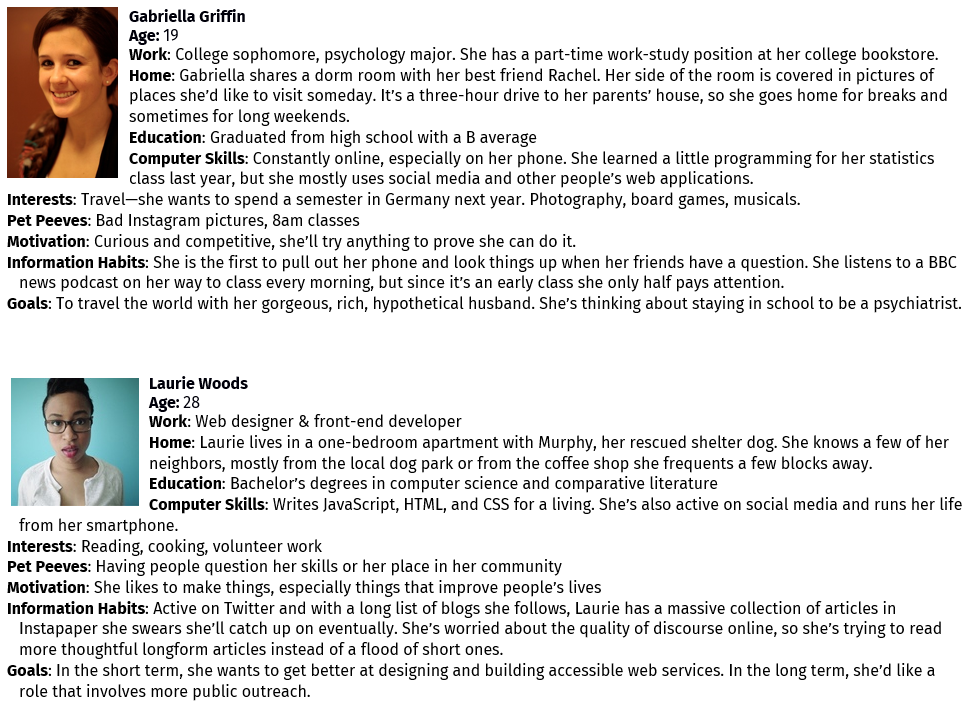
\includegraphics[width=0.95\textwidth]{personas}
  \caption{Primary Personas: Gabriella Griffin \& Laurie Woods}\label{fig:personas}
\end{figure}

\subsection{Tasks}\label{sec:design-tasks}
I do not assume viewers have any prior exposure to diversity statistics or to the tech industry. For users like Gabriella, the primary task the project supports is noticing the gender imbalance at all stages in the tech pipeline. Users like Laurie, who are already aware of the problem, can explore the statistics to see the extent of the problem. The project provides an overview of the data to give this high-level introduction to tech demographics, then presents each stage of the pipeline individually, allowing viewers to explore questions like:

\begin{itemize}
  \item When do women get involved in tech? Is a computer science degree required?
  \item Where does the pipeline leak? Is there a stage when more women seem to drop out?
  \item What kinds of technical careers are open to women? What kinds are still relatively closed?
  \item Does exposing girls to computer science at younger ages lead to more women working in IT\@?
\end{itemize}

The project should also answer questions about the importance of gender diversity in tech and about the interventions used to increase women's participation in IT\@. Some of this will come from the resources list, some from the narration.


\subsection{Design Goals}\label{sec:design-goals}
The webpage's design crucially needs to support exploring these kinds of questions, regardless of technical background or analytical skills. I focused on this need through several specific design goals:
\begin{description}
  \item[Overview first, with details on demand:] Adapted from \citet{Shneiderman1996Eyes}, this mantra of information visualization shaped the narrative structure of the project. Upon loading the webpage, viewers should immediately have an overview of women's participation along the tech education pipeline, with access to more detailed about each stage.
  \item[Consistency:] Detailed views of each stage in the pipeline should be presented consistently, to facilitate comparison of similar information across stages.
  \item[Use simple displays:] Data should be presented in familiar graphs wherever possible, so viewers can explore the data without being distracted by the form of the graph.
  \item[Guide interpretations:] Viewers without much background may have difficulty interpreting data, especially after the first few views. Use the narrative structure to guide viewers easily toward points of interest.
\end{description}


\subsection{Data Selection}\label{sec:design-data}
There are many sources of data on women in computing, from case studies of single computer science departments to occupation data at a national level. For the initial stage of this project, I chose to use publicly available datasets for each stage in the tech education pipeline that (a) include nation-wide data for the United States, (b) are cited in both the academic literature and in media reports, and (c) are structured similarly to aid in comparison across time stages. These criteria led me to three data sources, spanning high school education to industry employment.

\subsubsection*{The College Board's AP Computer Science Test Taker Demographics}
The College Board's Advanced Placement (AP) program offers high school students the opportunity to earn college credit for courses taken in high school by passing standardized exams. Each AP exam covers introductory college-level material within a single subject area. The exams are scored on a 1--5 scale, with scores 3--5 considered passing and eligible for college credit. AP exam data does not include students who are exposed to computing through other means, including the after-school programs that are popular interventions to introduce girls to coding. However, it provides consistent national data on the students who receive a rigorous introduction to computer science while in high school, and it is commonly used as a proxy for computing education before college.

\subsubsection*{The Annual Taulbee Survey of Diversity in Computing Education}
The nonprofit Computing Research Association (CRA) conducts and publishes the Taulbee Survey, an annual report on enrollment in computing programs in higher education. It reports on the number of students and faculty in computer science, computer engineering, and information departments across the United States, and gives demographic breakdowns for each education level. Because this project focuses on the traditional tech pipeline from high school to industry employment, I use the Taulbee data on bachelor's, master's, and PhD degrees awarded and exclude data on faculty and postdoctoral positions.

\subsubsection*{The Bureau of Labor Statistics' Employment Report by Occupation}
The United States Bureau of Labor Statistics posts detailed data by occupation as part of its Current Population Survey, broken down by gender and ethnicity. This includes a fairly granular section of ``Computing Occupations'', including specialties like database administration and web development.

These three sources are ideal for comparison for several reasons. First, they all have a national scope, avoiding the sample size problems of many single-department or regional case studies. Second, they are all regularly cited in existing research on diversity in tech and are publicly available for verification. Finally, they have a similar structure, with breakdowns by gender and by occupational or educational category. This makes them easy to present consistently, while allowing supplementary data to be added in the future to explore facets specific to that stage in the pipeline.


\section{Building the Visualization}\label{sec:methodology}
{\color{Magenta}
The increasing role of technology in society means that the questions the project explores---namely, who gets to build our technologies and how effective the calls for diversity in tech have been---are relevant to the general public, not merely to those inside the tech world. Consequently, the project has three major goals:
\begin{enumerate}
  \item Connect prior research by presenting data on both education and employment in tech
  \item Facilitate comparison across datasets, even for those without sophisticated analytical skills
  \item Provide context to highlight the importance of interesting points within the data
\end{enumerate}
}

\subsection{Data Collection \& Cleaning}\label{sec:dev-data}
As discussed in \autoref{sec:design-data}, I used AP exam data from the College Board\footnote{AP Demographics available at \url{https://research.collegeboard.org/programs/ap/data}}, graduation data from the Taulbee Survey\footnote{Taulbee Survey available at \url{http://cra.org/resources/taulbee-survey/}}, and employment data from the U.S. Bureau of Labor Statistics\footnote{Labor Statistics available at \url{https://www.bls.gov/cps/tables.htm}}
 to construct the visualizations. \autoref{tbl:data-sources} summarizes the subset of each dataset used for this project.

\begin{table}
  \begin{tabular}{L{3.6cm}cL{4cm}l} \hline
    \textbf{Data Source} & \textbf{Years Included} & \textbf{Subset} & \textbf{Variables} \\ \hline
    \href{https://research.collegeboard.org/programs/ap/data}{College Board AP Demographics}
      & 2010--2016
      & AP Computer Science Exam
      & Gender, Exam Score \\
    \href{http://cra.org/resources/taulbee-survey/}{CRA's Taulbee Survey}
      & 2010--2015
      & Graduate \& Undergraduate degrees awarded
      & Gender, Program \\
    \href{https://www.bls.gov/cps/tables.htm}{United States Bureau of Labor Statistics Detailed Employment (Table 11)}
      & 2011--2015
      & Computing Occupations
      & Gender, Occupation \\ \hline
  \end{tabular}
  \caption{Summary of Data Sources Used}\label{tbl:data-sources}
\end{table}

Where feasible, I collected all data going back to 2010; the Bureau of Labor Statistics changed their reporting categories in 2011, so for consistency I excluded their 2010 data. Only the College Board had released 2016 data at the time of collection. Because not all groups contain the same years' data, visualizations including multiple groups use percentage breakdowns by gender, rather than absolute numerical comparisons.

All three data sources are available either as spreadsheets or in PDF tables. The College Board spreadsheets include demographic information for all AP tests, broken out by gender and by exam score, so I extracted the data for the Computer Science exam and discarded the others. The Bureau of Labor Statistics similarly includes all occupations in their spreadsheet, so I extracted the data for all of the ``Computer and Mathematical Occupations'' as seen in the literature. The Taulbee Survey publishes its data as part of an annual PDF report; because the data is already aggregated (and consequently fairly small), I manually copied the data from their PDFs into a CSV file.

Both the College Board and the Taulbee Survey give the aggregated counts of male and female students for each relevant category, so the only further processing required was to format each row consistently. The Bureau of Labor Statistics, on the other hand, provides a total count of employees for each category, rounded to the nearest thousand, along with the percentage of women employed in each category. They do not provide diversity statistics for categories with fewer than 50,000 total employees, so I excluded these categories from the visualization. For the categories included, I used the percentages of female employees to calculate an approximate female employee count, to better correspond with the data for educational stages.

\subsection{Early Design Sketches}\label{sec:dev-sketches}
\begin{figure}
  \centering
  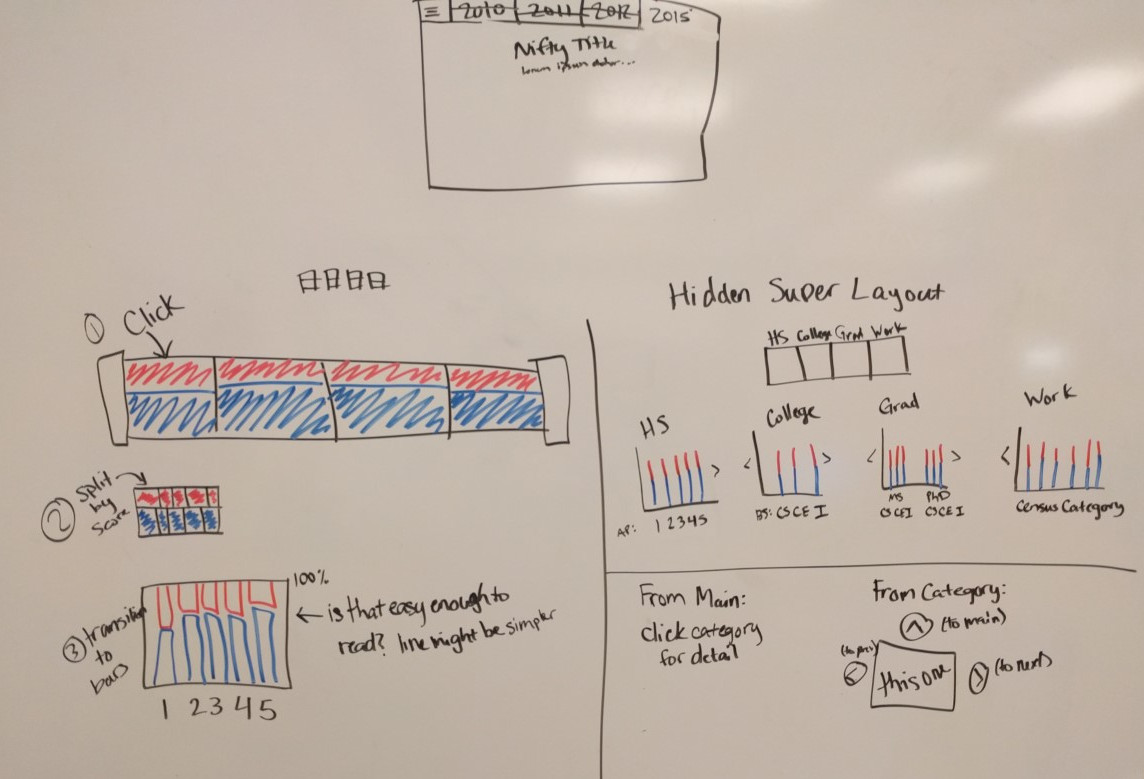
\includegraphics[width=0.8\textwidth]{whiteboard-1-layout}

  \vspace{0.1in}

  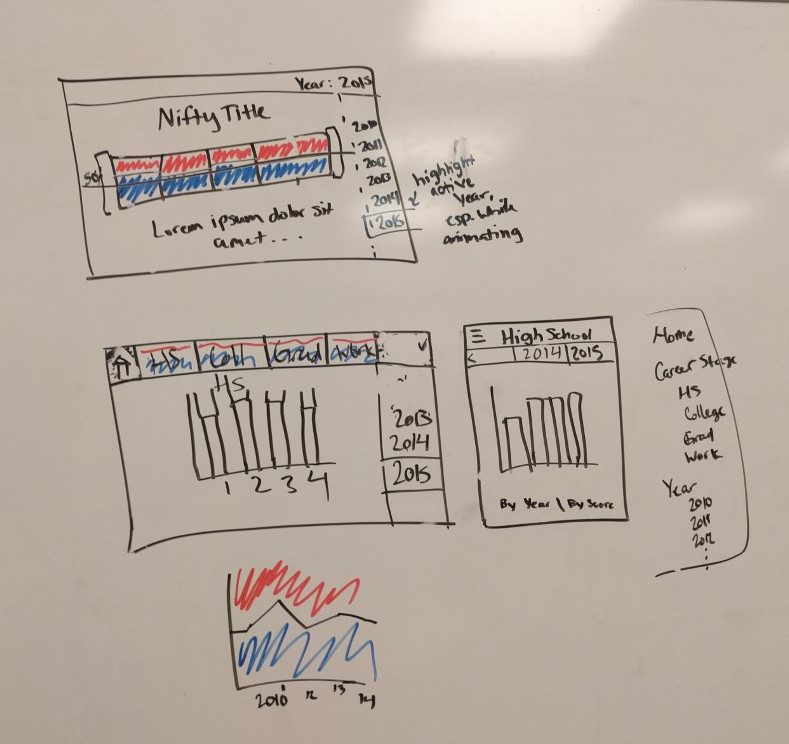
\includegraphics[width=0.8\textwidth]{whiteboard-2-navigation}
  \caption{Early Design Sketches: page layout (top) and alternate navigation (bottom)}\label{fig:whiteboard}
\end{figure}

I used low-fidelity whiteboard sketches to design and test early versions of the webpage before creating a code version. In the early designs, shown in \autoref{fig:whiteboard}, I focused on the visual relationship between the overview and the detailed views of each pipeline stage, on page navigation, and on graph types to display data. The top sketch shows disassembled overview of the page layout. The page frame at the top of the sketch uses a top navigation based on the stages of the tech education pipeline, so users interested in a particular stage can jump directly to it. To the left, it uses a pipe segment to visually represent the pipeline, which is divided into sections and color-coded according to the gender ratio of that section. The numbered sections below the pipe model a proposed animation from the overview into a bar graph for one of the detailed views. The right panel shows the spatial relationship between views, with vertical movement from the overview to each detailed view and horizontal movement between stages of the pipeline. This was intended to use the chronological nature of the pipeline to suggest a narrative on its own, connecting one stage of the pipeline to the next in the same way an individual would follow them throughout her career.

However, truly following the flow of a single career would require longitudinal data, which the combination of aggregated datasets cannot provide. Instead, the data supports viewing trends over time, so the bottom sketch explores ways to include time series information in the page navigation. The first panel introduces a drop-down menu to filter the entire display by year, with an option to animate through all available years. The next displays show alternatives for desktop and mobile views: on a large display, the top menu gets a series of colored backgrounds to mimic the color-coding of the overview pipe, with the same year filter as a dropdown. On smaller displays, the menu collapses into a hamburger pullout, and the year filter is present both within that menu and directly under the header, where it can be swiped sideways as needed. The bottom frame shows a color-coded area chart tracking the gender ratio over time.

The smudges in \autoref{fig:whiteboard} are evidence of my first round of testing, intended to determine whether the time-based navigation would make sense to viewers. Since this was a very preliminary test, I did not use rigorous standards for selecting participants or testing the layout: I asked nearby classmates who had no familiarity with my design goals if they would exchange feedback for a cookie. Two volunteered, so I brought them one at a time to the whiteboard, gave them a one-sentence introduction to the purpose of the site, and asked how they would interact with it. As they explained (or ``clicked'' on the whiteboard), I drew in details or menus, as needed.

Only one of the two found the drop-down without prompting, and she said she was unlikely to use a filter placed that far away from the graphs it applied to. The other participant simply wanted to scroll for more information.

\subsection{Refined Design Wireframes}\label{sec:dev-wireframes}
\begin{figure}
  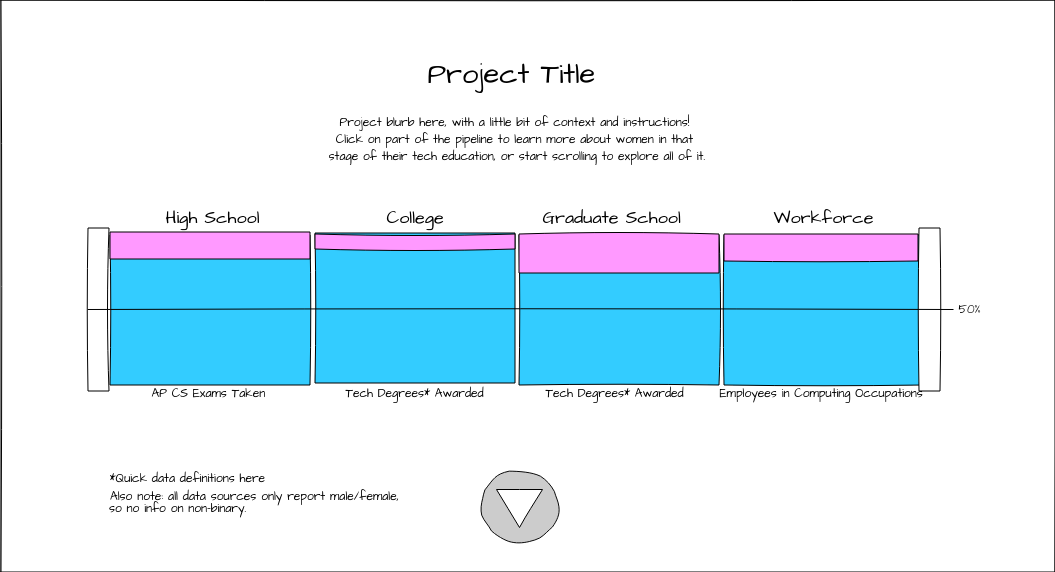
\includegraphics[width=\textwidth]{wireframe-1-overview}

  \vspace{2cm}

  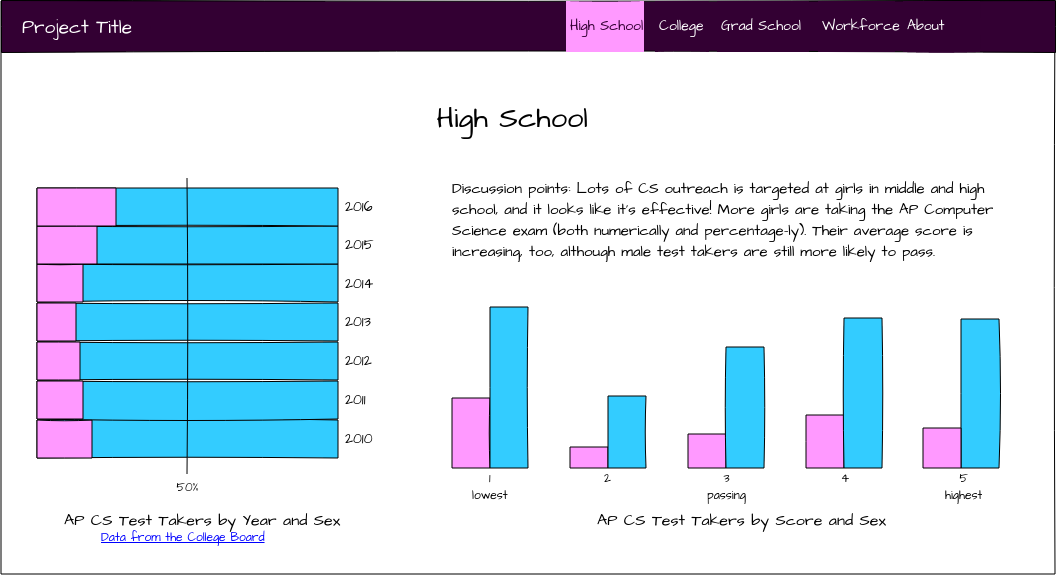
\includegraphics[width=\textwidth]{wireframe-2-hs-detail}
  \caption{Wireframes: overview (top) and high school detail (bottom)}\label{fig:wireframes}
\end{figure}

Since neither test participant found the time-based navigation useful, I removed it and simplified the page navigation for the next iteration of the design. Instead of a menu, viewers see a downward arrow indicating the page is scrollable; in this design, scrolling takes users from the overview to the detailed views, as well as from one detailed view to the next.

I also added narrative descriptions to each detailed view, to discuss issues unique to that stage in the pipeline and to highlight data of interest within that stage. I separated time series data and data by group (AP score, academic program, or specialized occupation) into two separate graphs, placed side-by-side, to show both the granular group data and the trends over time without relying on another menu. \autoref{fig:wireframes} shows the wireframes produced at the end of this refinement, made with the Pencil Prototyping tool\footnote{\url{http://pencil.evolus.vn/Next.html}}.

I performed another casual test at this point in the process, recruiting two new testers who roughly fit the personas presented in \autoref{sec:design-users}: a classmate interested in web development to represent Laurie's opinion, and an undergraduate communications major to represent Gabriella's. In addition to verifying that the simpler navigation was easier to understand, I used this test to compare ways of presenting the narrative elements. After explaining how they would interact with a page containing only the graphs and headings, they saw three different versions of the page: the same graphs-only layout, one with introductory text for each section, and one with annotations added to interesting points on the graph. The introductory texts were written on sticky notes and the annotations were on Post-It flags, so the two test layouts were of similar quality. Both testers preferred the version with introductory text pictured in the final wireframes, claiming the original version needed more explanation but that the annotations distracted from the graphs.


\subsection{Website Development}\label{sec:development}
\begin{figure}
  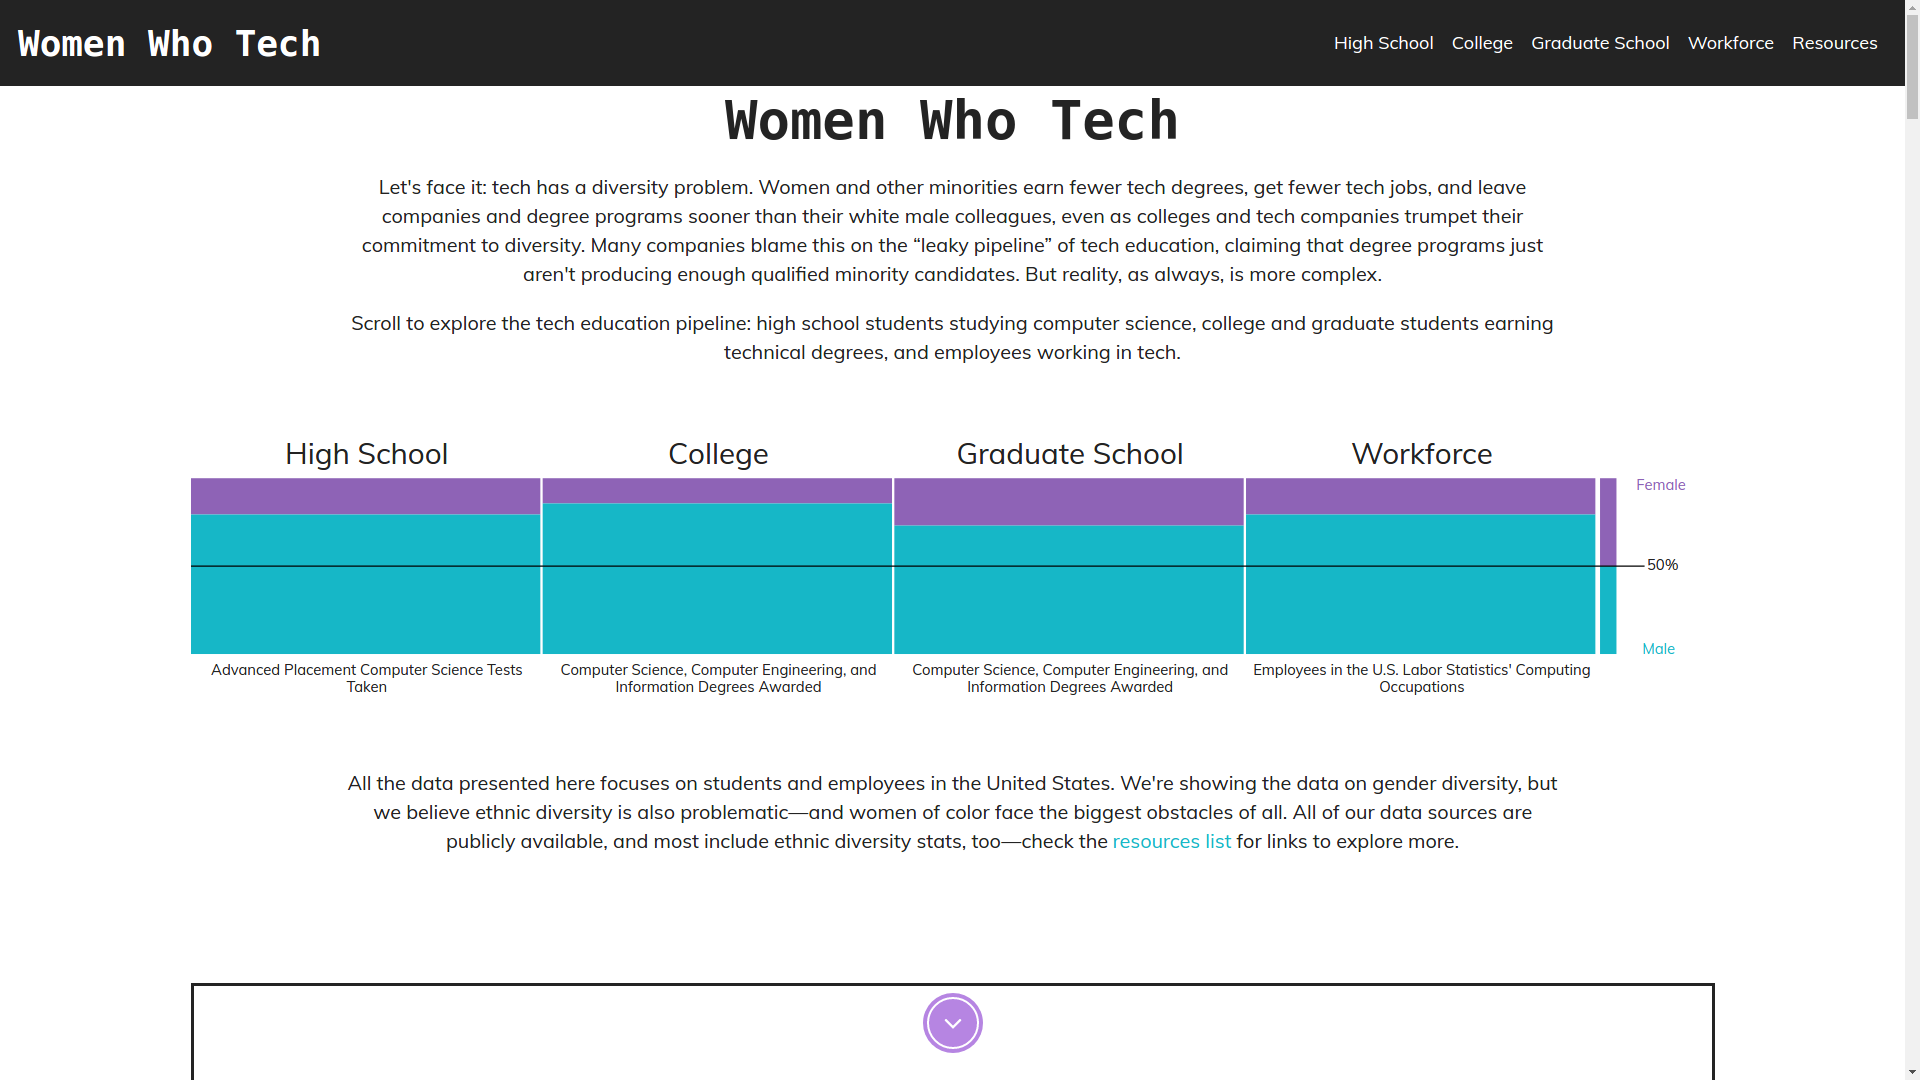
\includegraphics[width=0.95\textwidth]{screen-1-overview}


  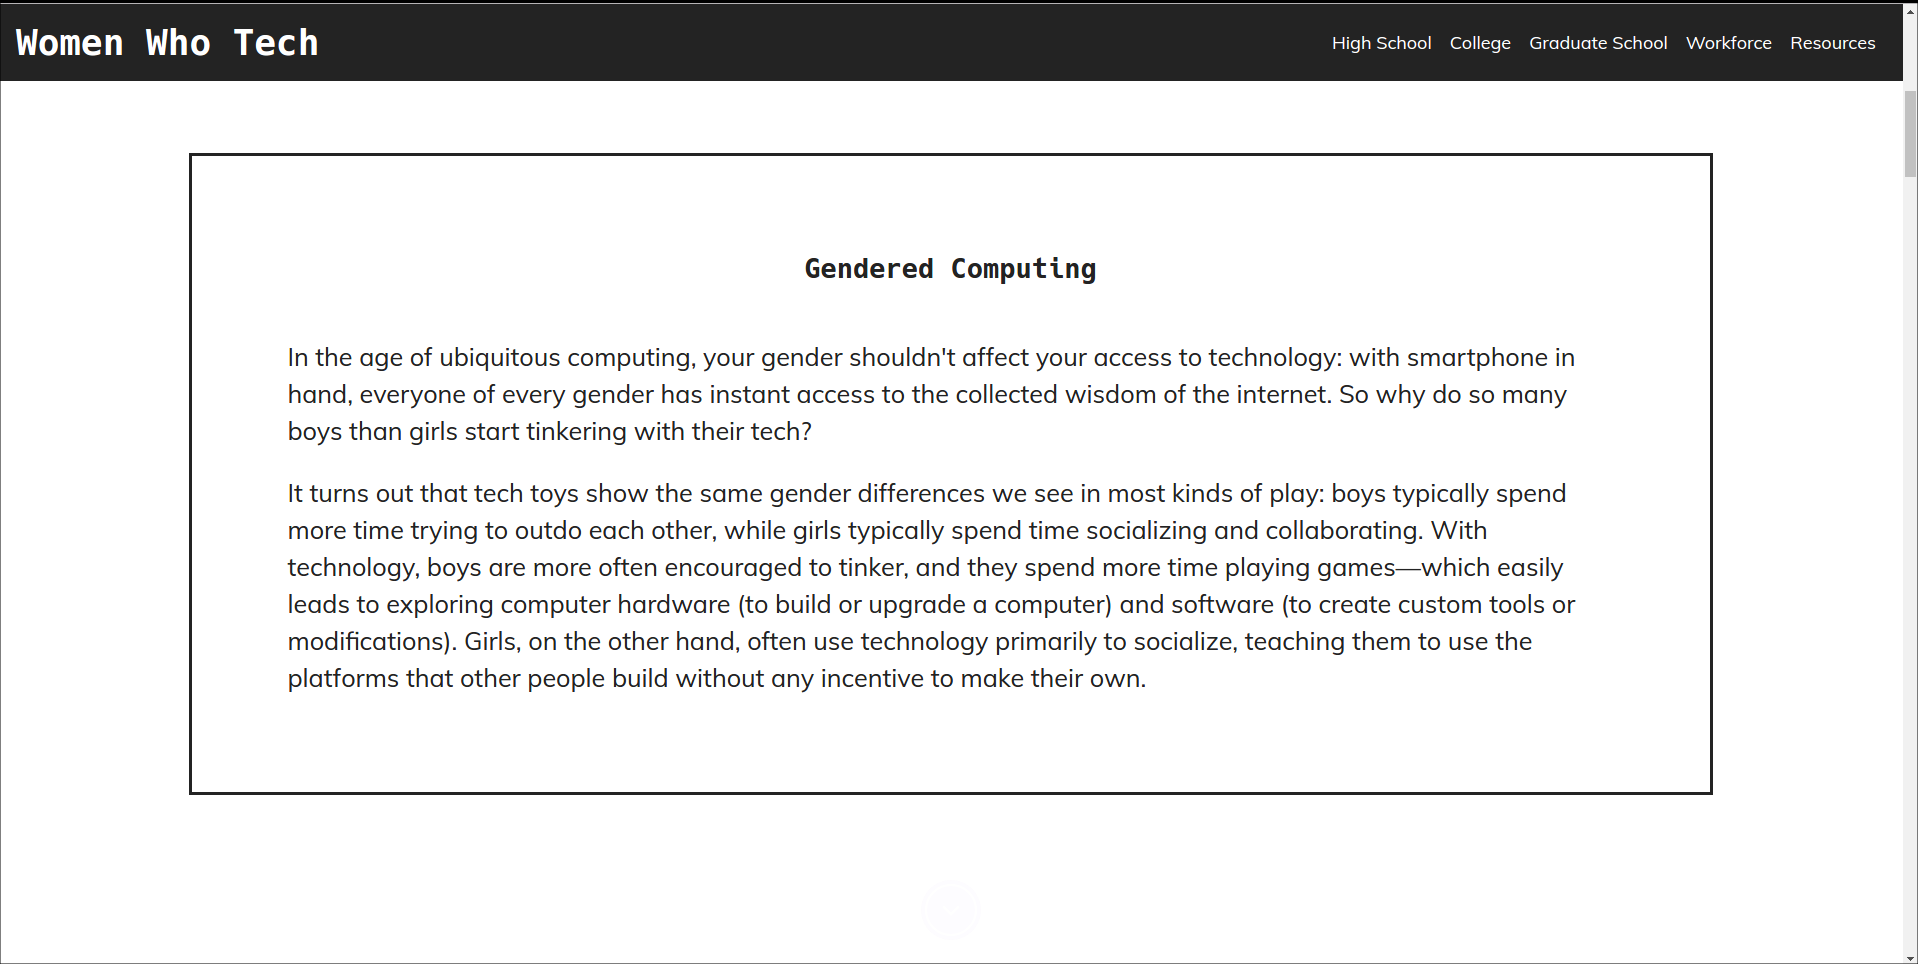
\includegraphics[width=0.95\textwidth]{screen-2-interlude}


  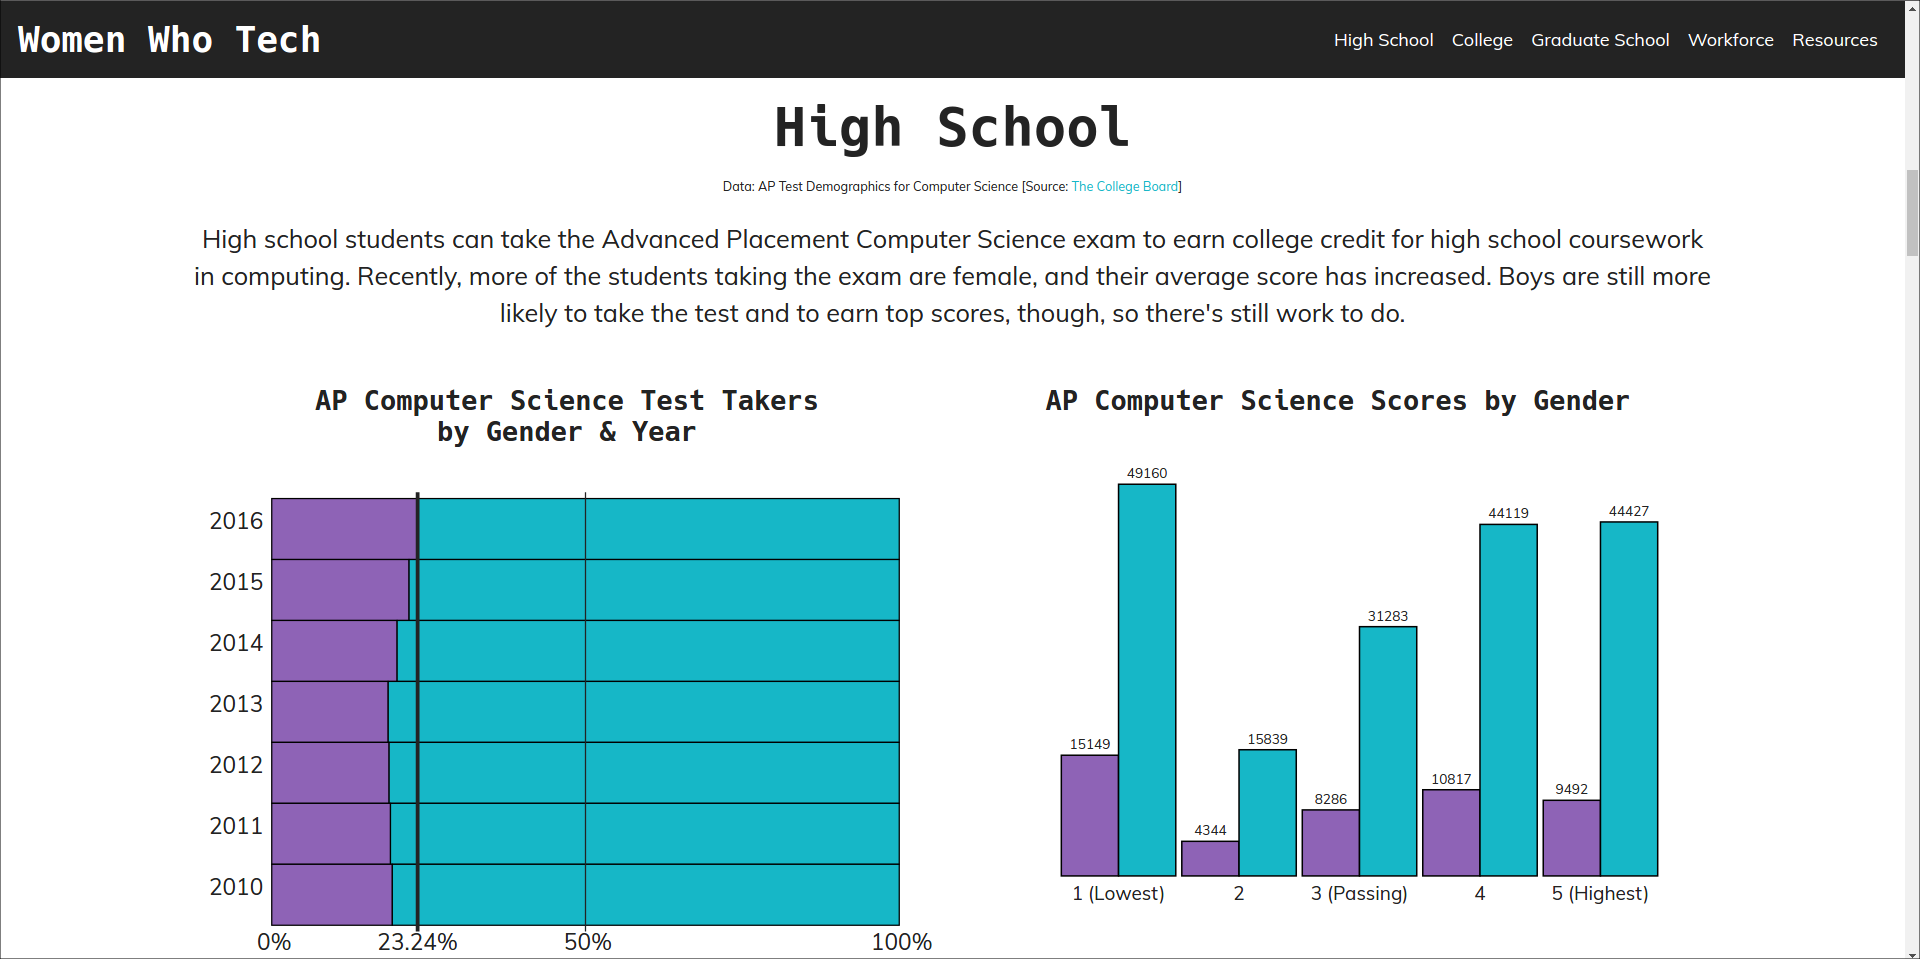
\includegraphics[width=0.95\textwidth]{screen-3-hs-detail}
  \caption{Screenshots: overview (top), narrative frame (middle), and high school detail (bottom)}\label{fig:screenshots}
\end{figure}

The actual webpage, shown in \autoref{fig:screenshots}, was constructed using HTML5/CSS3 for the page layout and the D3.js JavaScript library\footnote{\url{https://d3js.org/}} for the visualizations. The page display conforms to responsive web design principles, although the interactive aspects of the visualizations do not.

\textcolor{magenta}{EXPAND}


\section{User Testing}\label{sec:testing}
Throughout the design and development of the project, I collected feedback and incorporated it into later iterations. Two people offered feedback on the early design sketches and on the wireframes; I recruited a total of eight informal testers for the actual website, four loosely corresponding to each persona, to browse the site and offer their impressions. Some of the resulting changes were based on their explicit feedback, while others were based on my observations as they browsed. This section presents the major changes introduced during this process.

\subsection{Page Structure}
In several early wireframes, I included annotations directing viewers to points of interest directly on the graph. However, the users who saw these wireframes said the annotations felt cluttered and were less certain, not more, how to interpret the underlying data. This led to the narrative boxes in between graphical displays, providing similar context without infringing on graph space. However, later testers noted that these narrative frames are text-heavy and may be visually uninteresting to people who engage primarily with the visualizations; they may be a good place to bring in smaller, supplementary data sets to explore.

I also rearranged the detail views so that the introductory text is above the graphs, rather than next to the year graph as in the wireframes. This alleviated problems reading the category graph when bars were too short: the increased vertical space allowed for even short bars to be clearly visible.

\subsection{Navigation}
The menu bar on the top of the page jumps between primary sections---the data views along the pipeline---without displaying the narrative sections in between. Because the information is all contained on a single page, users have always been able to scroll to view all of the content. However, the earliest versions of the webpage did not have an indicator besides the native scrollbar that this was an option. Consequently, two of the first testers navigated the page entirely by clicking on the menu bar and never saw the narrative frames.

After observing these tests, I added a purple downward-pointing arrow to the top panel (seen in the top screenshot of \autoref{fig:screenshot}). It clearly indicates scrollability; all later testers scrolled down the page without difficulty. When viewers reach the first narrative frame, the arrow disappears to avoid obscuring later content. This did not cause further problems with navigation, presumably because by this point viewers had realized that scrolling was the easiest way to navigate the page.

\subsection{Future Improvements}
Testing also revealed areas for improvement that have not yet been addressed. Several testers commented that they would like to see more variation between groups: because high school and employment are very different life stages, people were interested in the different ways the lack of gender parity affects high schoolers and working adults. A popular suggestion was to include stories of girls and women affected directly, while two testers asked about the kinds of interventions used at each stage. One commented that she would like to see more variety in the section layouts, with more comparison features in the overview and unique displays for each set of details.

Another common request was for more time-oriented displays. While each detail display includes a summary of the data by year, the trends for all groups are never presented in the same view. Three of the eight testers asked for a time-specific overview, while one suggested animating the existing overview to show year-by-year changes. All four of these testers expressed a strong interest in an annotated timeline, showing changes in demographics along with the dates of big tech companies' diversity policies, nonprofit events, and other related milestones.


\section{Conclusion}\label{sec:conclusion}


% Bibliography
%------------------------------------------------------------------------------
\clearpage
\bigmargins
\bibliographystyle{apalike}
\bibliography{women-in-tech.bib}
%------------------------------------------------------------------------------


\end{document}
